\documentclass[12pt]{article}

\usepackage{sbc-template}

\usepackage{graphicx,url}

%\usepackage[brazil]{babel}   
%\usepackage[latin1]{inputenc}  
\usepackage[utf8]{inputenc}  
% UTF-8 encoding is recommended by ShareLaTex

     
\sloppy

\title{Doctoral Project Proposal: \\Bioinformatics Algorithms for Datacenter Networks}

\author{Iv{\'a}n Marcelo Carrera\inst{1}}


\address{Facultad de Ingenier{\'i}a de Sistemas -- Escuela Polit{\'e}cnica Nacional (EPN)\\
Ladr{\'o}n de Guevara E11-253. Quito -- Ecuador
  %\email{imci.carrera@gmail.com}
}

\begin{document} 

\maketitle

\begin{abstract}

This doctoral project proposal aims to present an overview of a research intended to be
\end{abstract}
     
\section{Introduction}

\section{Objectives}

\section{Concepts and State of Art}

\section{Potential Scientific Contributions}

%\section{Thesis Proposal}
%\section{Methodology}
%\subsection{Conferences and Journals}
%\section{Images}
\cite{mapreduce-revisited}

\bibliographystyle{sbc}
\bibliography{paper}

\end{document}

%\begin{figure}[ht]
%\centering
%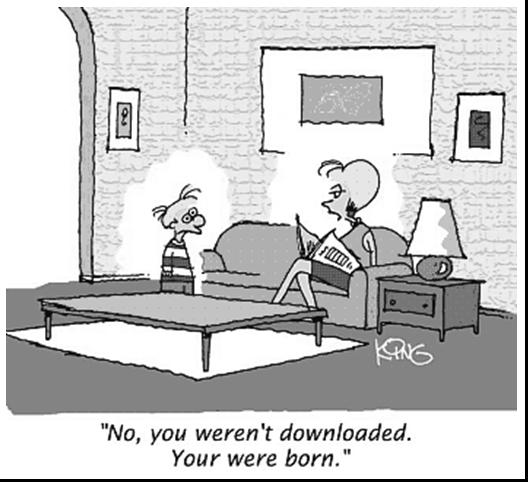
\includegraphics[width=.5\textwidth]{fig1.jpg}
%\caption{A typical figure}
%\label{fig:exampleFig1}
%\end{figure}
%
%\begin{figure}[ht]
%\centering
%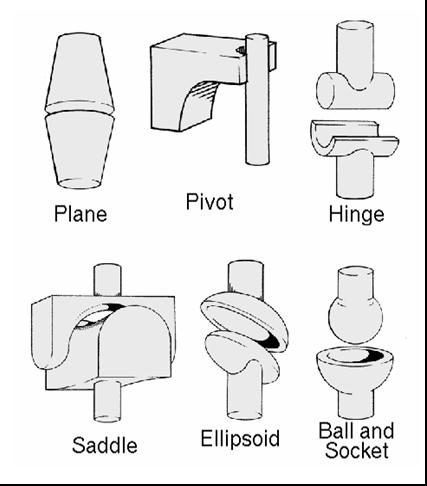
\includegraphics[width=.3\textwidth]{fig2.jpg}
%\caption{This figure is an example of a figure caption taking more than one
  %line and justified considering margins mentioned in Section~\ref{sec:figs}.}
%\label{fig:exampleFig2}
%\end{figure}

%\begin{table}[ht]
%\centering
%\caption{Variables to be considered on the evaluation of interaction
  %techniques}
%\label{tab:exTable1}
%\smallskip
%\begin{tabular}{|l|c|c|}
%\hline
%& Value 1 & Value 2\\[0.5ex]
%\hline
%&&\\[-2ex]
%Case 1 & 1.0 $\pm$ 0.1 & 1.75$\times$10$^{-5}$ $\pm$ 5$\times$10$^{-7}$\\[0.5ex]
%\hline
%&&\\[-2ex]
%Case 2 & 0.003(1) & 100.0\\[0.5ex]
%\hline
%\end{tabular}
%\end{table}